% questions.tex —— 2018 年·北京卷·文科 · 题目内容片段（无答案）
% 由 tools/generate_projects.py 依来源总账自 2018/2018_数学真题_北京卷文_试题.md 生成，勿手改（改源 MD 后重跑）


\gkpart{数学}

\begin{gktip}
按固定源印刷页码 1063—1064 转录。题 3、6、7、18 含图；图形依据固定源重绘。出版者、版次、上游来源链及官方身份未核；固定源未提供答案与解析。
\end{gktip}

\gkpart{一、选择题}

\begin{question}
\gkti{1}已知集合 $A=\{x\mid |x|<2\}$，$B=\{-2,0,1,2\}$，则 $A\cap B=$\mbox{（　　）}

（A）$\{0,1\}$　（B）$\{-1,0,1\}$　（C）$\{-2,0,1,2\}$　（D）$\{-1,0,1,2\}$

\end{question}
\begin{question}
\gkti{2}在复平面内，复数 $\dfrac{1}{1-\mathrm i}$ 的共轭复数对应的点位于\mbox{（　　）}

（A）第一象限　（B）第二象限　（C）第三象限　（D）第四象限

\Needspace{0.4\textheight}
\end{question}
\begin{question}
\gkti{3}执行如图所示的程序框图，输出的 $s$ 值为\mbox{（　　）}
\nopagebreak[4]
\begin{center}% 2018 北京卷文第3题：程序框图（据固定源第1063页重绘）
\begin{tikzpicture}[>=stealth, font=\small, node distance=5mm and 12mm]
  \tikzset{
    term/.style={draw, rounded corners=2pt, minimum width=12mm, minimum height=6mm, align=center},
    proc/.style={draw, minimum width=19mm, minimum height=7mm, align=center},
    test/.style={draw, diamond, aspect=2.5, inner sep=1pt, align=center},
    io/.style={draw, trapezium, trapezium left angle=70, trapezium right angle=110, minimum width=14mm, minimum height=6mm, align=center}
  }
  \node[term] (start) {开始};
  \node[proc, below=of start] (init) {$k=1,\ s=1$};
  \node[proc, below=of init, minimum width=31mm, minimum height=10mm] (sum) {$s=s+(-1)^k\cdot\dfrac{1}{1+k}$};
  \node[proc, below=of sum] (inc) {$k=k+1$};
  \node[test, below=of inc, minimum width=17mm, minimum height=7mm] (cond) {$k\ge3$};
  \node[io, below=of cond] (out) {输出 $s$};
  \node[term, below=of out] (end) {结束};
  \draw[->] (start)--(init);
  \draw[->] (init)--(sum);
  \draw[->] (sum)--(inc);
  \draw[->] (inc)--(cond);
  \draw[->] (cond)--node[right]{是}(out);
  \draw[->] (out)--(end);
  \draw[->] (cond.east)--node[above]{否} ++(12mm,0)|-(sum.east);
\end{tikzpicture}
\end{center}
\nopagebreak[4]
（A）$\dfrac12$　（B）$\dfrac56$　（C）$\dfrac76$　（D）$\dfrac7{12}$

\end{question}
\begin{question}
\gkti{4}设 $a,b,c,d$ 是非零实数，则“$ad=bc$”是“$a,b,c,d$ 成等比数列”的\mbox{（　　）}

（A）充分而不必要条件　（B）必要而不充分条件\\
（C）充分必要条件　（D）既不充分也不必要条件

\end{question}
\begin{question}
\gkti{5}“十二平均律”是通用的音律体系，明代朱载堉最早用数学方法计算出半音比例，为这个理论的发展做出了重要贡献。十二平均律将一个纯八度音程分成十二份，依次得到十三个单音，从第二个单音起，每一个单音的频率与它的前一个单音的频率的比都等于 $\sqrt[12]{2}$。若第一个单音的频率为 $f$，则第八个单音的频率为\mbox{（　　）}

（A）$\sqrt[3]{2}f$　（B）$\sqrt[3]{2^2}f$　（C）$\sqrt[12]{2^5}f$　（D）$\sqrt[12]{2^7}f$

\Needspace{0.4\textheight}
\end{question}
\begin{question}
\gkti{6}某四棱锥的三视图如图所示，在此四棱锥的侧面中，直角三角形的个数为\mbox{（　　）}
\nopagebreak[4]
\begin{center}% 2018 北京卷文第6题：四棱锥三视图（据固定源第1063页重绘）
\begin{tikzpicture}[font=\small, line cap=round, line join=round]
  % 正（主）视图：高2，底边分为两个单位段，投影线从顶点落至分点
  \begin{scope}
    \draw (0,0)--(2,0)--(0,2)--cycle;
    \draw (0,2)--(1,0);
    \draw[<->] (-0.18,0)--(-0.18,2) node[midway,left] {$2$};
    \draw[<->] (0,-0.18)--(1,-0.18) node[midway,below] {$1$};
    \draw[<->] (1,-0.18)--(2,-0.18) node[midway,below] {$1$};
    \node[below=7mm] at (1,0) {正（主）视图};
  \end{scope}
  % 侧（左）视图
  \begin{scope}[xshift=3.4cm]
    \draw (0,0)--(2,0)--(0,2)--cycle;
    \draw[<->] (0,-0.18)--(2,-0.18) node[midway,below] {$2$};
    \node[below=7mm] at (1,0) {侧（左）视图};
  \end{scope}
  % 俯视图：梯形外轮廓，底边收敛为下方中点及左下点
  \begin{scope}[yshift=-2.9cm]
    \draw (0,0)--(0,1.5)--(2,1.5)--(1,0)--cycle;
    \draw (0,1.5)--(1,0);
    \node[below=2mm] at (1,0) {俯视图};
  \end{scope}
\end{tikzpicture}
\end{center}
\nopagebreak[4]
（A）$1$　（B）$2$　（C）$3$　（D）$4$

\Needspace{0.4\textheight}
\end{question}
\begin{question}
\gkti{7}在平面直角坐标系中，$\widehat{AB}$、$\widehat{CD}$、$\widehat{EF}$、$\widehat{GH}$ 是圆 $x^2+y^2=1$ 上的四段弧（如图），点 $P$ 在其中一段上，角 $\alpha$ 以 $Ox$ 为始边，$OP$ 为终边。若 $\tan\alpha<\cos\alpha<\sin\alpha$，则 $P$ 所在的圆弧是\mbox{（　　）}
\nopagebreak[4]
\begin{center}% 2018 北京卷文第7题：单位圆上的四段候选弧（据固定源第1063页重绘）
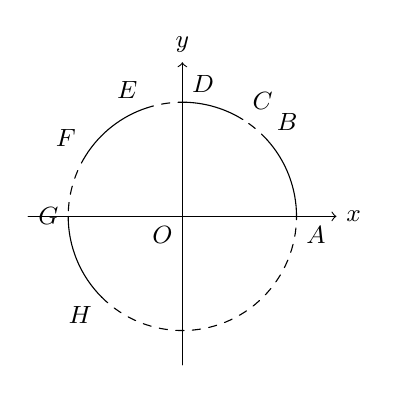
\begin{tikzpicture}[scale=1.45, font=\small, line cap=round]
  \draw[->] (-1.35,0)--(1.35,0) node[right] {$x$};
  \draw[->] (0,-1.3)--(0,1.35) node[above] {$y$};
  % 仅四段候选弧为实线；其余圆周分段画虚线
  \draw (1,0) arc (0:42:1);
  \draw[dashed] (42:1) arc (42:58:1);
  \draw (58:1) arc (58:88:1);
  \draw[dashed] (88:1) arc (88:108:1);
  \draw (108:1) arc (108:148:1);
  \draw[dashed] (148:1) arc (148:180:1);
  \draw (180:1) arc (180:225:1);
  \draw[dashed] (225:1) arc (225:360:1);
  \node[below left] at (0,0) {$O$};
  \node[below right] at (1,0) {$A$};
  \node[above right] at (42:1) {$B$};
  \node[above right] at (58:1) {$C$};
  \node[above right] at (0,1) {$D$};
  \node[above left] at (108:1) {$E$};
  \node[above left] at (148:1) {$F$};
  \node[left] at (180:1) {$G$};
  \node[below left] at (225:1) {$H$};
\end{tikzpicture}
\end{center}
\nopagebreak[4]
（A）$\widehat{AB}$　（B）$\widehat{CD}$　（C）$\widehat{EF}$　（D）$\widehat{GH}$

\end{question}
\begin{question}
\gkti{8}设集合 $A=\{(x,y)\mid x-y\ge1,\ ax+y>4,\ x-ay\le2\}$，则\mbox{（　　）}

（A）对任意实数 $a$，$(2,1)\in A$　（B）对任意实数 $a$，$(2,1)\notin A$

（C）当且仅当 $a<0$ 时，$(2,1)\notin A$　（D）当且仅当 $a\le\dfrac32$ 时，$(2,1)\notin A$

\end{question}
\gkpart{二、填空题}

\begin{question}
\gkti{9}设向量 $\boldsymbol a=(1,0)$，$\boldsymbol b\;(-1,m)$。若 $\boldsymbol a\perp(m\boldsymbol a-\boldsymbol b)$，则 $m=$\gkblank{}。

\begin{gktip}
第9题固定源在 $\boldsymbol b$ 与 $(-1,m)$ 之间未印等号；此处保留原貌，待核。
\end{gktip}

\end{question}
\begin{question}
\gkti{10}已知直线 $l$ 过点 $(1,0)$ 且垂直于 $x$ 轴。若 $l$ 被抛物线 $y^2=4ax$ 截得的线段长为 $4$，则抛物线的焦点坐标为\gkblank{}。

\end{question}
\begin{question}
\gkti{11}能说明“若 $a>b$，则 $\dfrac1a<\dfrac1b$”为假命题的一组 $a,b$ 的值依次为\gkblank{}。

\end{question}
\begin{question}
\gkti{12}若双曲线 $\dfrac{x^2}{a^2}-\dfrac{y^2}{4}=1\ (a>0)$ 的离心率为 $\dfrac{\sqrt5}{2}$，则 $a=$\gkblank{}。

\end{question}
\begin{question}
\gkti{13}若 $x,y$ 满足 $x+1\le y\le2x$，则 $2y-x$ 的最小值是\gkblank{}。

\end{question}
\begin{question}
\gkti{14}若 $\triangle ABC$ 的面积为 $\dfrac{\sqrt3}{4}(a^2+c^2-b^2)$，且 $\angle C$ 为钝角，则 $\angle B=$\gkblank{}；$\dfrac ca$ 的取值范围是\gkblank{}。

\end{question}
\gkpart{三、解答题}

\begin{question}
\gkti{15}设 $\{a_n\}$ 是等差数列，且 $a_1=\ln2$，$a_2+a_3=5\ln2$。

（1） 求 $\{a_n\}$ 的通项公式；

（2） 求 $\mathrm e^{a_1}+\mathrm e^{a_2}+\cdots+\mathrm e^{a_n}$。

\end{question}
\begin{question}
\gkti{16}已知函数 $f(x)=\sin^2x+\sqrt3\sin x\cos x$。

（1） 求 $f(x)$ 的最小正周期；

（2） 若 $f(x)$ 在区间 $\left[-\dfrac\pi3,m\right]$ 上的最大值为 $\dfrac32$，求 $m$ 的最小值。

\end{question}
\begin{question}
\gkti{17}电影公司随机收集了电影的有关数据，经分类整理得到下表：

\begin{center}
\begin{tabular}{crrrrrr}
\toprule
电影类型 & 第一类 & 第二类 & 第三类 & 第四类 & 第五类 & 第六类 \\
\midrule
电影部数 & 140 & 50 & 300 & 200 & 800 & 510 \\
好评率 & 0.4 & 0.2 & 0.15 & 0.25 & 0.2 & 0.1 \\
\bottomrule
\end{tabular}
\end{center}

好评率是指：一类电影中获得好评的部数与该类电影的部数的比值。

（1） 从电影公司收集的电影中随机选取 1 部，求这部电影是获得好评的第四类电影的概率；

（2） 随机选取 1 部电影，估计这部电影没有获得好评的概率；

（3） 电影公司为增加投资回报，拟改变投资策略，这将导致不同类型电影的好评率发生变化。假设表格中只有两类电影的好评率数据发生变化，那么哪类电影的好评率增加 0.1，哪类电影的好评率减少 0.1，使得获得好评的电影总部数与样本中的电影总部数的比值达到最大？（只需写出结论）

\Needspace{0.4\textheight}
\end{question}
\begin{question}
\gkti{18}如图，在四棱锥 $P-ABCD$ 中，底面 $ABCD$ 为矩形，平面 $PAD\perp$ 平面 $ABCD$，$PA\perp PD$，$PA=PD$，$E,F$ 分别为 $AD,PB$ 的中点。
\nopagebreak[4]
\begin{center}% 2018 北京卷文第18题：四棱锥与中点（据固定源第1064页重绘）
\begin{tikzpicture}[font=\small, line cap=round, line join=round]
  % 投影位置按原图透视关系布置
  \coordinate (A) at (0,0);
  \coordinate (B) at (1.5,-0.35);
  \coordinate (C) at (4.2,0.05);
  \coordinate (D) at (2.7,0.55);
  \coordinate (P) at (1.25,3.0);
  \coordinate (E) at ($(A)!0.5!(D)$);
  \coordinate (F) at ($(P)!0.5!(B)$);
  % 矩形底面：后边 AD、DC 为虚线，前侧为实线
  \draw (A)--(B)--(C);
  \draw[dashed] (C)--(D)--(A);
  % 侧棱：遮挡棱以虚线表示
  \draw (P)--(A) (P)--(B) (P)--(C);
  \draw[dashed] (P)--(D);
  % 原图标示 P--E 为虚线；不绘制 E--F
  \draw[dashed] (P)--(E);
  \fill (A) circle (1.1pt) (B) circle (1.1pt) (C) circle (1.1pt) (D) circle (1.1pt)
        (P) circle (1.1pt) (E) circle (1.1pt) (F) circle (1.1pt);
  \node[above] at (P) {$P$};
  \node[left] at (A) {$A$};
  \node[below] at (B) {$B$};
  \node[right] at (C) {$C$};
  \node[right] at (D) {$D$};
  \node[below left] at (E) {$E$};
  \node[right] at (F) {$F$};
\end{tikzpicture}
\end{center}
\nopagebreak[4]
（1） 求证：$PE\perp BC$；

（2） 求证：平面 $PAB\perp$ 平面 $PCD$；

（3） 求证：$EF\parallel$ 平面 $PCD$。

\end{question}
\begin{question}
\gkti{19}设函数 $f(x)=[ax^2-(3a+1)x+3a+2]\mathrm e^x$。

（1） 若曲线 $y=f(x)$ 在点 $(2,f(2))$ 处的切线斜率为 $0$，求 $a$；

（2） 若 $f(x)$ 在 $x=1$ 处取得极小值，求 $a$ 的取值范围。

\end{question}
\begin{question}
\gkti{20}已知椭圆 $M:\dfrac{x^2}{a^2}+\dfrac{y^2}{b^2}=1\ (a>b>0)$ 的离心率为 $\dfrac{\sqrt6}{3}$，焦距为 $2\sqrt2$，斜率为 $k$ 的直线 $l$ 与椭圆 $M$ 有两个不同的交点 $A,B$。

（1） 求椭圆 $M$ 的方程；

（2） 若 $k=1$，求 $|AB|$ 的最大值；

（3） 设 $P(-2,0)$，直线 $PA$ 与椭圆 $M$ 的另一个交点为 $C$，直线 $PB$ 与椭圆 $M$ 的另一个交点为 $D$。若 $C,D$ 和点 $Q\left(-\dfrac74,\dfrac14\right)$ 共线，求 $k$。

\end{question}